\documentclass[11pt]{article}
% Suggested arXiv categories: cs.AI (primary), cs.GT (secondary)

% Encoding & typography
\usepackage[T1]{fontenc}
\usepackage[utf8]{inputenc}
\usepackage{lmodern}
\usepackage[margin=1in]{geometry}
\usepackage{microtype}

% Math / tables / figures
\usepackage{amsmath,amssymb}
\usepackage{booktabs}
\usepackage{graphicx}
\usepackage{caption}

% Links / lists / authors
\usepackage[hidelinks]{hyperref}
\usepackage{enumitem}
\usepackage{authblk}
\usepackage{tikz}
\usepackage{pgfplots}
\pgfplotsset{compat=1.18}
\usepackage{fancyvrb}
\usepackage[table]{xcolor}

\newcommand{\tOne}{T001}
\newcommand{\tTwo}{T002}

\title{Moreau Arena: How Adaptation and Exact Formulas Transform LLM Strategic Reasoning from Systematic Failure to Baseline-Beating Performance}

\author[1]{Victor Stasiuc}
\affil[1]{Independent Researcher\\
\texttt{stvitek@gmail.com}\\
ORCID: \href{https://orcid.org/0009-0003-2064-0486}{0009-0003-2064-0486}}

\date{February 2026}

\begin{document}
\maketitle

\vspace{-0.7em}
\begin{abstract}
Moreau Arena is a contamination-resistant benchmark for strategic reasoning: agents must design a ``build'' (an animal plus a discrete stat allocation) for a novel, stochastic combat game whose rules are specified only in the prompt.
We evaluate the same set of 13 agents (8 frontier LLMs, 5 non-LLM baselines) in two tournaments that differ only in the information and feedback scaffolding provided.

Tournament~001 (\tOne) runs 779 completed best-of-7 series (3652 total games) under a one-shot, blind-pick protocol with qualitative ability descriptions.
Baselines dominate: the top three agents are all non-LLM baselines, and LLMs win only 37.50\% of LLM-vs-baseline series.
We identify a qualitative failure mode---the ``WIL trap''---where some LLMs systematically over-invest in willpower despite its low marginal utility under the true game mechanics.

Tournament~002 (\tTwo) reruns the same round-robin (780 series; 4015 games) but removes key confounds: we provide exact numerical formulas, inject meta context (top-performing builds), enforce structured JSON outputs, and allow per-game adaptation (the loser sees the winner's build and may re-pick).
The results flip: by Bradley--Terry (BT) ranking, all LLMs outrank all baselines, and LLMs win 89.75\% of LLM-vs-baseline series.
GPT-5.2-Codex achieves the largest BT gain ($+0.881$, rank~9$\to$1), while the strongest \tOne baselines fall to the bottom five.
Despite this reversal, adaptation is not a universal solution: across all LLM agents, changing builds after a loss yields 51.06\% win rate in subsequent games, and several high-performing models win primarily by finding strong builds early rather than counter-picking game-by-game.
We also observe non-transitive matchups in \tTwo (12 strict 3-cycles; none in \tOne), indicating that with feedback, the meta supports genuine rock--paper--scissors dynamics.

\textbf{Scope and contribution.}
Taken together, the two tournaments show that LLM strategic performance in this setting is limited less by ``raw capability'' than by comprehension and feedback: with vague rules and no adaptation, LLMs pattern-match archetypes; with exact mechanics, examples, and feedback, they reliably surpass handcrafted baselines.
We release complete prompts, configuration hashes, match records, and analysis code to support reproducibility.
\end{abstract}

\section{Introduction}

Large language models (LLMs) increasingly act as decision-makers in interactive settings: recommending actions, planning under uncertainty, and adapting to opponents.
Yet evaluating strategic reasoning is difficult: many benchmarks are either too static (single-step questions) or too contaminated (popular games and well-known strategies).

We introduce \textbf{Moreau Arena}, a compact, synthetic strategy benchmark designed to stress quantitative trade-offs while minimizing training-data leakage.
An agent chooses one of six animals offered in the prompt (bear, buffalo, boar, monkey, tiger, wolf) and allocates 20 stat points across health (HP), attack (ATK), speed (SPD), and willpower (WIL).
The game then simulates stochastic combat under fixed rules.
(The underlying simulator supports additional species for internal testing; one baseline, RandomAgent, samples from the full roster and happens to select \texttt{raven} under its fixed seed.)

This paper reports a controlled comparison of \textbf{two tournaments with identical agents, game configuration, and match schedule, but different information scaffolding}.
The core question is not ``can LLMs play the game'' but \emph{what conditions let LLMs express strategic competence}.
Tournament~001 (\tOne) is intentionally under-specified (qualitative abilities; no feedback), exposing systematic failure modes.
Tournament~002 (\tTwo) removes confounds by providing exact formulas, injecting meta knowledge, requiring structured outputs, and enabling per-game adaptation.

\subsection*{Contributions}

This paper contributes:
\begin{enumerate}[leftmargin=*]
\item A newly authored game environment (Moreau Arena) designed to reduce contamination risk and to admit a derivable dominant strategy under a frozen configuration snapshot.
\item Two 13-agent round-robin tournaments (8 frontier LLMs, 5 baselines), totaling 1559 best-of-7 series under different information scaffolding regimes.
\item Evidence that the \tOne$\to$\tTwo performance reversal---from baseline dominance to LLM dominance---implicates comprehension and feedback rather than an absence of strategic capability.
\item Characterization of consistent failure modes (the WIL trap, low build diversity) and of when adaptation helps versus when fast convergence suffices.
\end{enumerate}

\section{Related Work}

\paragraph{Strategic agents and games.}
CICERO~\cite{cicero} combines language models with planning to achieve strong play in Diplomacy, while Pluribus~\cite{pluribus} demonstrates superhuman play in multiplayer poker.
Such games are strategically rich, but they are heavily documented, increasing the likelihood that modern LLMs have seen strategies or transcripts during training.

\paragraph{Game-based benchmarks.}
The NetHack Learning Environment (NLE)~\cite{nle} and procedurally generated RL benchmarks~\cite{procgen} aim to measure generalization in challenging domains.
These environments are not primarily designed to test whether a model can derive an optimal strategy from a compact rulesheet without interaction or learning.

\paragraph{Reasoning benchmarks.}
Widely used datasets such as MMLU~\cite{mmlu}, GSM8K~\cite{gsm8k}, BIG-bench~\cite{bigbench}, and ARC~\cite{arc} test isolated reasoning skills, often in non-adversarial settings.
They do not directly measure one-shot \emph{strategic} reasoning where a single decision must integrate multiple mechanics under competition.

\paragraph{Evaluation methodology.}
Preference-based leaderboards such as LMSYS Chatbot Arena~\cite{chatbot_arena} and broad evaluation suites such as HELM~\cite{helm} provide useful comparative signals but depend on human judgments and may conflate helpfulness with capability.
Moreau Arena uses objective win/loss outcomes from a seeded simulator and paired-comparison modeling.
We adopt Bradley--Terry ranking~\cite{bradley_terry}, widely used for paired outcomes, as our primary metric and include Elo only as a secondary, path-dependent score.

\section{Moreau Arena}

\paragraph{Game core.}
Each agent selects (i) one animal from the prompt roster and (ii) a stat allocation with HP+ATK+SPD+WIL=20 (each $\ge 1$).
Animals provide passives and a low-probability special ability; outcomes are stochastic due to random ability procs and tie-break rules.
A ``series'' is first-to-4 wins (best-of-7 in decisive games), but drawn games can occur and do not increment the score, so the number of simulated games per series can exceed~7.
Matches take place on an 8$\times$8 grid for at most 60 ticks; a closing ring begins at tick~30 and damages creatures on outer tiles, shrinking the safe zone to 4$\times$4 by tick~40.

\paragraph{Why ATK stacking is a derivable dominant strategy.}
The stat formulas are:
\[
\texttt{max\_hp} = 50 + 10\cdot \texttt{HP},\qquad
\texttt{base\_dmg} = \left\lfloor 2 + 0.85\cdot \texttt{ATK}\right\rfloor,
\]
\[
\texttt{dodge} = \min(30\%, 2.5\%\cdot \texttt{SPD}),\qquad
\texttt{resist} = \min(60\%, 3.3\%\cdot \texttt{WIL}).
\]
ATK=14 yields base\_dmg=13, while ATK=8 yields 8---a 62.5\% increase for 6 points.
By comparison, 6 points of HP add only 60 max HP, often insufficient to offset faster time-to-kill under ring pressure.
Proc rates (3.5--4.5\% per tick) are low enough that proc-focused or resistance-focused allocations have small expected value.

\paragraph{Contamination resistance.}
The animals, abilities, and numerical parameters are bespoke to this benchmark.
Agents cannot rely on memorized openings or known metas; they must infer trade-offs from the prompt (\tOne) or apply explicit mechanics (\tTwo).

\paragraph{Auto-balancer (benchmark as a living test).}
A common failure mode in synthetic strategy benchmarks is ``overfitting the ruleset'': once a single dominant build is found, the benchmark collapses into a static lookup task.
Moreau Arena includes an \emph{auto-balancer} that can be enabled between tournaments to keep the meta non-stationary.
After each tournament, each animal's empirical win rate is tracked with an exponential moving average (EMA) with smoothing $\alpha=0.15$.
Proc probabilities are then nudged by a small multiplicative adjustment with coefficient $\beta=0.03$ in the direction that reduces deviation from a target 50\% win rate, with clipping to keep parameters in a valid range:
\[
\mathrm{EMA}_{t+1} = \alpha w_t + (1-\alpha)\mathrm{EMA}_t,\qquad
p_{t+1} = \mathrm{clip}\!\left(p_t\left(1+\beta(0.5-\mathrm{EMA}_t)\right)\right).
\]
This makes the benchmark a repeated-game setting rather than a one-and-done puzzle.
\textbf{In this paper, the auto-balancer is disabled and the game configuration is frozen across \tOne and \tTwo} to isolate prompting and feedback effects.

\section{Experimental Setup}
\label{sec:setup}

\subsection{Agents}

We evaluate 13 agents: eight frontier LLMs and five non-LLM baselines.

\paragraph{LLMs.} Claude Opus 4.6, Claude Sonnet 4.6, Claude Haiku 4.5 (Anthropic);
GPT-5.2 and GPT-5.2 Codex (OpenAI);
Gemini 3 Flash and Gemini 3.1 Pro (Google);
Grok 4.1 Fast (xAI).

\paragraph{Baselines.}
\emph{SmartAgent} performs internal simulation (200 match rollouts) over a candidate build set and selects the empirically best build; in \tTwo it re-evaluates candidates after observing the winner's build, producing up to 5 distinct builds across its series.
\emph{HighVarianceAgent} hard-codes the glass-cannon build \texttt{bear 3/14/2/1} (verified identical in both tournaments).
\emph{ConservativeAgent} hard-codes a high-HP buffalo build (\texttt{buffalo 8/6/4/2}).
\emph{GreedyAgent} uses a hand-written lookup policy (\texttt{boar 8/8/3/1}).
\emph{RandomAgent} samples from the full simulator roster under a fixed seed, producing \texttt{raven 3/3/2/12} deterministically; it serves as a floor baseline and does not affect conclusions (0--120 series record in both tournaments).

\subsection{Tournament protocols}

Both tournaments use the same round-robin schedule over all $\binom{13}{2}=78$ pairings, with 10 independent series per pairing (780 planned series).

\paragraph{Tournament 001 (\tOne): one-shot blind pick.}
Agents receive qualitative descriptions of animals and abilities (Appendix~\ref{app:t1_prompt}) and output a single build per series.
Agents do not observe opponent choices or results during build selection.
\tOne contains 779 completed series due to one runtime error in a single pairing.

\paragraph{Tournament 002 (\tTwo): exact formulas + meta + per-game adaptation.}
\tTwo adds four major interventions simultaneously:
(1) exact numerical formulas for damage, procs, and ring mechanics;
(2) meta context in the prompt (top-performing builds automatically extracted from \tOne match records; see Appendix~\ref{app:t2_prompt} for the exact injected text);
(3) structured JSON output constrained by a per-provider schema;
(4) per-game adaptation within each series---after each game, the loser sees the winner's build and may re-pick, while the winner's build is locked.

Meta context was extracted automatically by filtering out floor baselines (RandomAgent, HighVarianceAgent) and ranking remaining builds by win rate on the filtered subset.
All five injected builds showed 100\% win rate on their filtered subsamples (4--22 games each), though game-level win rates across all agents are lower (80--100\%; see Appendix~\ref{app:t2_prompt}).

\begin{table}[h]
\centering
\small
\caption{Summary of protocol differences between tournaments.}
\label{tab:protocol}
\begin{tabular}{p{0.45\columnwidth} p{0.45\columnwidth}}
\toprule
Tournament~001 & Tournament~002 \\
\midrule
One-shot per series & Per-game adaptation (loser repicks; winner locked) \\
Blind pick & Loser sees opponent animal+stats \\
Qualitative ability text & Exact numerical formulas \\
No meta context & Top-5 builds injected from \tOne \\
Free-text output & Strict JSON schema per provider \\
\bottomrule
\end{tabular}
\end{table}

\subsection{Metrics}

We report:
(i) Bradley--Terry (BT) scores fit to pairwise series outcomes, normalized to $[0,1]$ with 95\% bootstrap confidence intervals;
(ii) Elo ratings computed over series outcomes as an auxiliary perspective;
(iii) series win--loss totals from the round-robin;
(iv) build diversity (unique builds used) and adaptation metrics in \tTwo.

\section{Tournament 001 Results: One-Shot Strategy Failure}

\subsection{Baselines dominate}

Table~\ref{tab:t1_rank} and Figure~\ref{fig:t1_bt} summarize \tOne.
The top three ranks are occupied by non-LLM baselines (SmartAgent, HighVarianceAgent, ConservativeAgent), while the best LLM (Gemini Flash) ranks 4th with BT=0.503.
LLMs win only 150/400=37.50\% of LLM-vs-baseline series.

\begin{table}[t]
\centering
\small
\caption{Tournament~001 rankings by Bradley--Terry (BT) score with 95\% bootstrap confidence intervals, plus Elo and series records.}
\label{tab:t1_rank}
\begin{tabular}{rllclrr}
\toprule
Rank & Agent & Type & BT (95\% CI) & Elo & W--L & Ser. \\
\midrule
1 & SmartAgent & Base & 1.000 [.610, 1.000] & 1672 & 99--21 & 120 \\
2 & HighVariance & Base & 0.954 [.555, 1.000] & 1632 & 98--22 & 120 \\
3 & Conservative & Base & 0.643 [.372, .917] & 1780 & 89--31 & 120 \\
4 & Gemini Flash & LLM & 0.503 [.267, .771] & 1718 & 83--37 & 120 \\
5 & Gemini Pro & LLM & 0.455 [.247, .678] & 1682 & 80--39 & 119 \\
6 & Grok-4.1 Fast & LLM & 0.437 [.230, .665] & 1865 & 79--40 & 119 \\
7 & Greedy & Base & 0.239 [.128, .346] & 1362 & 64--56 & 120 \\
8 & GPT-5.2 & LLM & 0.230 [.122, .343] & 1439 & 63--57 & 120 \\
9 & GPT-5.2-Codex & LLM & 0.119 [.067, .168] & 1477 & 47--73 & 120 \\
10 & Cl.\ Sonnet 4.6 & LLM & 0.066 [.034, .097] & 1528 & 34--86 & 120 \\
11 & Cl.\ Haiku 4.5 & LLM & 0.056 [.030, .081] & 1396 & 31--89 & 120 \\
12 & Cl.\ Opus 4.6 & LLM & 0.017 [.009, .024] & 1194 & 12--108 & 120 \\
13 & Random & Base & 0.005 [.003, .008] & 757 & 0--120 & 120 \\
\bottomrule
\end{tabular}
\end{table}

\begin{figure}[t]
\centering
\begin{tikzpicture}
\begin{axis}[
xbar,
xmin=0, xmax=1.05,
height=9cm,
width=\columnwidth,
xlabel={BT score},
ytick={0,1,2,3,4,5,6,7,8,9,10,11,12},
yticklabels={Smart,HV,Cons,Flash,GPro,Grok,Greedy,GPT,Codex,Sonnet,Haiku,Opus,Rand},
y dir=reverse,
bar width=6pt,
error bars/.cd, x dir=both, x explicit,
]
\addplot+[error bars/.cd, x dir=both, x explicit] coordinates {
(1.0000,0) +- (0.3900,0.0000)
(0.9541,1) +- (0.3995,0.0459)
(0.6426,2) +- (0.2708,0.2744)
(0.5028,3) +- (0.2359,0.2686)
(0.4553,4) +- (0.2088,0.2229)
(0.4373,5) +- (0.2075,0.2272)
(0.2388,6) +- (0.1111,0.1068)
(0.2296,7) +- (0.1079,0.1129)
(0.1193,8) +- (0.0528,0.0482)
(0.0656,9) +- (0.0320,0.0317)
(0.0564,10) +- (0.0263,0.0241)
(0.0173,11) +- (0.0079,0.0069)
(0.0054,12) +- (0.0024,0.0024)
};
\addplot[black,dashed] coordinates {(0,2.5) (1.05,2.5)};
\end{axis}
\end{tikzpicture}
\caption{Tournament~001 BT scores with 95\% bootstrap confidence intervals. Dashed line marks the boundary below the top-3 baselines (ranks 1--3).}
\label{fig:t1_bt}
\end{figure}

\subsection{Pairwise structure}

The pairwise matrix (Table~\ref{tab:t1_matrix}) shows a largely transitive hierarchy: we find 0 strict 3-cycles where $A$ beats $B$, $B$ beats $C$, and $C$ beats $A$ (all edges $>$50\%).

\subsection{The WIL trap}

The most consistent and costly failure mode is over-investing in WIL.
Claude Opus is the extreme case: it repeats \texttt{wolf 3/8/1/8} in 85.8\% of series and averages WIL$\approx$7.9.
The \tOne prompt describes resistance as $\texttt{resist}=\min(60\%,3.3\%\cdot\texttt{WIL})$, which can appear large in isolation.
However, under the simulator mechanics, resist applies only to ability procs, whose base probability is 3.5--4.5\% per tick.
Even under a generous upper bound (4.5\% base proc rate), at WIL=8 the expected number of resisted procs over a 60-tick match is
\[
60 \times 0.045 \times 0.264 \approx 0.71,
\]
i.e., fewer than one blocked proc per match.
This is typically not worth sacrificing multiple points of ATK (large, reliable damage) or SPD (initiative and dodge).
Across the 8 LLMs, mean WIL is strongly negatively correlated with BT (Spearman $\rho=-0.93$, $p<0.001$), consistent with WIL acting as a systematic trap rather than a nuanced trade-off.

\subsection{Build patterns and diversity}

Table~\ref{tab:t1_build} summarizes build choices in \tOne.
Baselines are effectively fixed-build agents (unique builds$\le$2), while LLMs vary widely in exploration.
Among LLMs, build diversity correlates strongly with performance (Spearman $\rho=0.81$, $p=0.015$), suggesting that searching the build space from vague rules is a key bottleneck.

\subsection{The price paradox}

Claude models are the weakest LLM family in \tOne.
Opus is worst overall among LLMs (BT=0.017) despite being the most expensive Claude tier, while Sonnet is the strongest Claude in this tournament (BT=0.066).
The price ordering across Claude tiers (Opus $>$ Sonnet $>$ Haiku) does not predict performance ordering, suggesting that helpfulness-oriented tuning and stylistic polish do not imply stronger quantitative strategy derivation under one-shot constraints.

\begin{table}[t]
\centering
\footnotesize
\caption{Tournament~001 build patterns. ``Unique builds'' counts distinct (animal, HP, ATK, SPD, WIL) tuples across all series.}
\label{tab:t1_build}
\begin{tabular}{llcrrl}
\toprule
Agent & Top animal & Avg stats & UA & UB & Signature \\
\midrule
SmartAgent & Bear 100\% & 3/14/2/1 & 1 & 1 & bear 3/14/2/1 \\
HighVar & Bear 100\% & 3/14/2/1 & 1 & 1 & bear 3/14/2/1 \\
Conserv & Buffalo 100\% & 8/6/4/2 & 1 & 1 & buffalo 8/6/4/2 \\
Flash & Tiger 51\% & 6.4/8.8/3.6/1.2 & 4 & 53 & bear 8/10/1/1 (13\%) \\
GPro & Tiger 73\% & 6.6/8.6/3.6/1.2 & 3 & 21 & tiger 6/8/5/1 (16\%) \\
Grok & Bear 42\% & 6.2/8.1/4.3/1.4 & 6 & 60 & bear 8/8/3/1 (19\%) \\
Greedy & Boar 100\% & 8/8/3/1 & 1 & 1 & boar 8/8/3/1 \\
GPT & Tiger 61\% & 7.3/7.0/3.8/1.9 & 2 & 19 & tiger 6/8/5/1 (38\%) \\
Codex & Tiger 87\% & 5.9/7.2/5.1/1.8 & 4 & 37 & tiger 6/7/5/2 (29\%) \\
Sonnet & Wolf 99\% & 4/8/5.2/2.7 & 2 & 3 & wolf 4/8/5/3 (73\%) \\
Haiku & Tiger 68\% & 5.3/7.3/5/2.4 & 2 & 9 & tiger 4/7/6/3 (54\%) \\
Opus & Wolf 100\% & 3/8.1/1/7.9 & 1 & 2 & wolf 3/8/1/8 (86\%) \\
Random & Raven 100\% & 3/3/2/12 & 1 & 1 & raven 3/3/2/12 \\
\bottomrule
\end{tabular}
\vspace{0.3em}
\noindent\footnotesize{UA = unique animals; UB = unique builds.}
\end{table}

\begin{table}[t]
\centering
\footnotesize
\setlength{\tabcolsep}{2.5pt}
\renewcommand{\arraystretch}{1.05}
\caption{Tournament~001 pairwise series win rates (\%). Most matchups use 10 series; Gemini~Pro vs Grok uses 9 due to one runtime error.}
\label{tab:t1_matrix}
\begin{tabular}{lrrrrrrrrrrrrr}
\toprule
 & Sm & HV & Co & Fl & GP & Gr & Gy & G5 & Cx & So & Ha & Op & Ra \\
\midrule
Sm & -- & 60 & 100 & 70 & 60 & 60 & 70 & 70 & 100 & 100 & 100 & 100 & 100 \\
HV & 40 & -- & 100 & 50 & 70 & 60 & 90 & 70 & 100 & 100 & 100 & 100 & 100 \\
Co & 0 & 0 & -- & 60 & 60 & 80 & 100 & 90 & 100 & 100 & 100 & 100 & 100 \\
Fl & 30 & 50 & 40 & -- & 50 & 50 & 80 & 80 & 80 & 90 & 80 & 100 & 100 \\
GP & 40 & 30 & 40 & 50 & -- & 22 & 60 & 70 & 90 & 100 & 100 & 100 & 100 \\
Gr & 40 & 40 & 20 & 50 & 78 & -- & 70 & 80 & 70 & 50 & 100 & 100 & 100 \\
Gy & 30 & 10 & 0 & 20 & 40 & 30 & -- & 50 & 80 & 80 & 100 & 100 & 100 \\
G5 & 30 & 30 & 10 & 20 & 30 & 20 & 50 & -- & 70 & 70 & 100 & 100 & 100 \\
Cx & 0 & 0 & 0 & 20 & 10 & 30 & 20 & 30 & -- & 100 & 60 & 100 & 100 \\
So & 0 & 0 & 0 & 10 & 0 & 50 & 20 & 30 & 0 & -- & 30 & 100 & 100 \\
Ha & 0 & 0 & 0 & 20 & 0 & 0 & 0 & 0 & 40 & 70 & -- & 80 & 100 \\
Op & 0 & 0 & 0 & 0 & 0 & 0 & 0 & 0 & 0 & 0 & 20 & -- & 100 \\
Ra & 0 & 0 & 0 & 0 & 0 & 0 & 0 & 0 & 0 & 0 & 0 & 0 & -- \\
\bottomrule
\end{tabular}
\vspace{0.3em}
\noindent\footnotesize{Sm=SmartAgent, HV=HighVariance, Co=Conservative, Fl=Flash, GP=Gemini Pro, Gr=Grok, Gy=Greedy, G5=GPT-5.2, Cx=Codex, So=Sonnet, Ha=Haiku, Op=Opus, Ra=Random.}
\end{table}

\section{Tournament 002 Results: Scaffolding Flips the Leaderboard}

\subsection{Rankings flip: LLMs outrank all baselines}

Table~\ref{tab:t2_rank} and Figure~\ref{fig:t2_bt} show \tTwo.
By BT score, all eight LLM agents rank above all five baselines.
The group-level reversal is stark: LLMs win 89.75\% of LLM-vs-baseline series in \tTwo, up from 37.50\% in \tOne.

\begin{table}[t]
\centering
\small
\caption{Tournament~002 rankings by Bradley--Terry (BT) score with 95\% bootstrap confidence intervals, plus Elo and series records.}
\label{tab:t2_rank}
\begin{tabular}{rllclrr}
\toprule
Rank & Agent & Type & BT (95\% CI) & Elo & W--L & Ser. \\
\midrule
1 & GPT-5.2-Codex & LLM & 1.000 [.793, 1.000] & 1879 & 104--16 & 120 \\
2 & Gemini Flash & LLM & 0.679 [.393, 1.000] & 1672 & 96--24 & 120 \\
3 & Grok-4.1 Fast & LLM & 0.650 [.366, 1.000] & 1900 & 95--25 & 120 \\
4 & Cl.\ Opus 4.6 & LLM & 0.252 [.143, .393] & 1526 & 71--49 & 120 \\
5 & Cl.\ Sonnet 4.6 & LLM & 0.252 [.130, .427] & 1709 & 71--49 & 120 \\
6 & GPT-5.2 & LLM & 0.252 [.140, .422] & 1758 & 71--49 & 120 \\
7 & Cl.\ Haiku 4.5 & LLM & 0.226 [.127, .359] & 1553 & 68--52 & 120 \\
8 & Gemini Pro & LLM & 0.188 [.104, .311] & 1527 & 63--57 & 120 \\
9 & SmartAgent & Base & 0.093 [.049, .147] & 1336 & 44--76 & 120 \\
10 & HighVariance & Base & 0.070 [.038, .108] & 1335 & 37--83 & 120 \\
11 & Conservative & Base & 0.061 [.031, .103] & 1286 & 34--86 & 120 \\
12 & Greedy & Base & 0.043 [.021, .076] & 1262 & 26--94 & 120 \\
13 & Random & Base & 0.007 [.004, .010] & 757 & 0--120 & 120 \\
\bottomrule
\end{tabular}
\end{table}

\begin{figure}[t]
\centering
\begin{tikzpicture}
\begin{axis}[
xbar,
xmin=0, xmax=1.05,
height=9cm,
width=\columnwidth,
xlabel={BT score},
ytick={0,1,2,3,4,5,6,7,8,9,10,11,12},
yticklabels={Codex,Flash,Grok,Opus,Sonnet,GPT,Haiku,GPro,Smart,HV,Cons,Greedy,Rand},
y dir=reverse,
bar width=6pt,
error bars/.cd, x dir=both, x explicit,
]
\addplot+[error bars/.cd, x dir=both, x explicit] coordinates {
(1.0000,0) +- (0.2075,0.0000)
(0.6793,1) +- (0.2863,0.3207)
(0.6496,2) +- (0.2840,0.3504)
(0.2520,3) +- (0.1091,0.1414)
(0.2520,4) +- (0.1223,0.1746)
(0.2520,5) +- (0.1122,0.1697)
(0.2258,6) +- (0.0989,0.1334)
(0.1882,7) +- (0.0839,0.1226)
(0.0926,8) +- (0.0436,0.0539)
(0.0698,9) +- (0.0319,0.0383)
(0.0614,10) +- (0.0306,0.0415)
(0.0426,11) +- (0.0217,0.0335)
(0.0066,12) +- (0.0028,0.0035)
};
\addplot[black,dashed] coordinates {(0,7.5) (1.05,7.5)};
\end{axis}
\end{tikzpicture}
\caption{Tournament~002 BT scores with 95\% bootstrap confidence intervals. Dashed line separates LLMs (above) from baselines (below).}
\label{fig:t2_bt}
\end{figure}

\subsection{The new top tier: Codex, Flash, Grok}

\tTwo exhibits a clear top tier.
GPT-5.2-Codex ranks 1st (BT=1.000), Gemini Flash 2nd (BT=0.679), and Grok 3rd (BT=0.650).
There is a large gap from rank~3 to rank~4: BT drops from 0.650 to 0.252.
Pairwise, Grok beats Flash in 9/10 series (Table~\ref{tab:t2_matrix}) yet loses to Codex 2--8, illustrating the non-transitive dynamics that emerge under adaptation.

\subsection{Rank reshuffling across tournaments}

Table~\ref{tab:t1_t2_comp} and Figure~\ref{fig:rank_slope} summarize rank changes.
The \tTwo winner, GPT-5.2-Codex, achieves the largest BT gain ($+0.881$), jumping from rank~9 in \tOne to rank~1 in \tTwo.
Conversely, \tOne winner SmartAgent falls from rank~1 to rank~9 ($\Delta$BT=$-$0.907).
Claude Opus improves dramatically (BT 0.017$\to$0.252; a 14.6$\times$ increase) and ties for the largest rank jump ($+$8, shared with Codex), but remains the weakest Claude by Elo and still loses 0--10 to Claude Sonnet in both tournaments.

Three agents (Opus, Sonnet, GPT-5.2) share BT=0.252 in \tTwo; ordering among them is not statistically resolved.
We list them in the order returned by the BT fit and report Elo as an auxiliary metric.

\begin{table}[t]
\centering
\small
\caption{Tournament~001 vs Tournament~002 comparison. Positive $\Delta$Rank indicates improvement (lower rank number).}
\label{tab:t1_t2_comp}
\begin{tabular}{llrrrr}
\toprule
Agent & Type & R\textsubscript{T1} & R\textsubscript{T2} & $\Delta$R & $\Delta$BT \\
\midrule
GPT-5.2-Codex & LLM & 9 & 1 & +8 & +0.881 \\
Gemini Flash & LLM & 4 & 2 & +2 & +0.177 \\
Grok-4.1 Fast & LLM & 6 & 3 & +3 & +0.212 \\
Cl.\ Opus 4.6 & LLM & 12 & 4 & +8 & +0.235 \\
Cl.\ Sonnet 4.6 & LLM & 10 & 5 & +5 & +0.186 \\
GPT-5.2 & LLM & 8 & 6 & +2 & +0.022 \\
Cl.\ Haiku 4.5 & LLM & 11 & 7 & +4 & +0.169 \\
Gemini Pro & LLM & 5 & 8 & $-$3 & $-$0.267 \\
SmartAgent & Base & 1 & 9 & $-$8 & $-$0.907 \\
HighVariance & Base & 2 & 10 & $-$8 & $-$0.884 \\
Conservative & Base & 3 & 11 & $-$8 & $-$0.581 \\
Greedy & Base & 7 & 12 & $-$5 & $-$0.196 \\
Random & Base & 13 & 13 & 0 & +0.001 \\
\bottomrule
\end{tabular}
\end{table}

\begin{figure}[t]
\centering
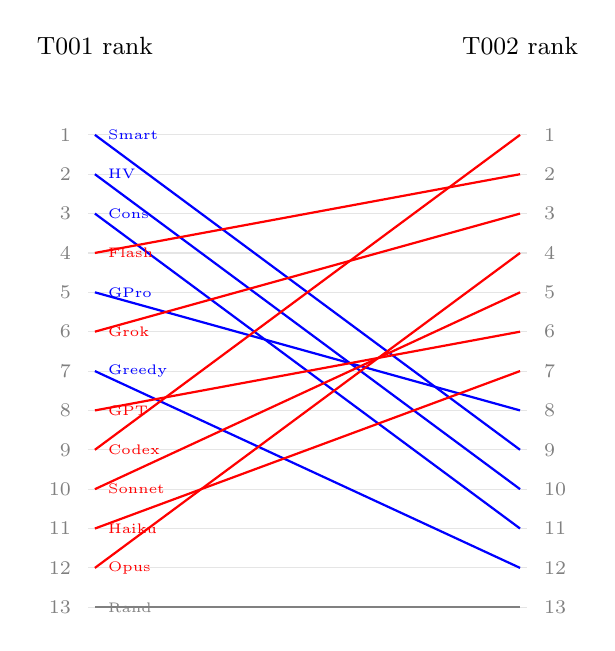
\begin{tikzpicture}[x=0.9cm,y=0.5cm]
\node[anchor=south,font=\small] at (0,0.8) {\tOne{} rank};
\node[anchor=south,font=\small] at (6,0.8) {\tTwo{} rank};
\foreach \i in {1,...,13} {
  \node[anchor=east,gray,font=\scriptsize] at (-0.2,-\i) {\i};
  \node[anchor=west,gray,font=\scriptsize] at (6.2,-\i) {\i};
  \draw[gray!20] (-0.1,-\i) -- (6.1,-\i);
}
\draw[thick,blue] (0,-1) -- (6,-9); \node[anchor=west,blue,font=\tiny] at (0.05,-1) {Smart};
\draw[thick,blue] (0,-2) -- (6,-10); \node[anchor=west,blue,font=\tiny] at (0.05,-2) {HV};
\draw[thick,blue] (0,-3) -- (6,-11); \node[anchor=west,blue,font=\tiny] at (0.05,-3) {Cons};
\draw[thick,red] (0,-4) -- (6,-2); \node[anchor=west,red,font=\tiny] at (0.05,-4) {Flash};
\draw[thick,blue] (0,-5) -- (6,-8); \node[anchor=west,blue,font=\tiny] at (0.05,-5) {GPro};
\draw[thick,red] (0,-6) -- (6,-3); \node[anchor=west,red,font=\tiny] at (0.05,-6) {Grok};
\draw[thick,blue] (0,-7) -- (6,-12); \node[anchor=west,blue,font=\tiny] at (0.05,-7) {Greedy};
\draw[thick,red] (0,-8) -- (6,-6); \node[anchor=west,red,font=\tiny] at (0.05,-8) {GPT};
\draw[thick,red] (0,-9) -- (6,-1); \node[anchor=west,red,font=\tiny] at (0.05,-9) {Codex};
\draw[thick,red] (0,-10) -- (6,-5); \node[anchor=west,red,font=\tiny] at (0.05,-10) {Sonnet};
\draw[thick,red] (0,-11) -- (6,-7); \node[anchor=west,red,font=\tiny] at (0.05,-11) {Haiku};
\draw[thick,red] (0,-12) -- (6,-4); \node[anchor=west,red,font=\tiny] at (0.05,-12) {Opus};
\draw[thick,gray] (0,-13) -- (6,-13); \node[anchor=west,gray,font=\tiny] at (0.05,-13) {Rand};
\end{tikzpicture}
\caption{Rank changes from \tOne to \tTwo (lower is better). Red: improved; blue: dropped; gray: unchanged.}
\label{fig:rank_slope}
\end{figure}

\subsection{Adaptation: when does feedback help?}

\tTwo allows the loser of each game to re-pick after seeing the winner's build.
Table~\ref{tab:t2_adapt} reports per-model adaptation propensity, build diversity, and post-loss outcomes conditional on adapting vs.\ sticking.

Across the eight LLMs, adaptation is common (1065 adaptations over 1591 losses; 66.9\%).
When an LLM agent changes its build after a loss, it wins 51.06\% of subsequent games; when it does not change, it wins 31.84\%.
However, adaptation rate is only weakly correlated with final BT (Spearman $\rho=0.19$ across LLMs), suggesting that finding strong builds early is often more important than reactive counter-picking.
Gemini Flash exemplifies this: it adapts in only 38\% of losses but achieves a 76\% win rate when it does, compared to 37\% when it sticks---it found strong builds fast and did not need to change often.

\begin{table}[t]
\centering
\footnotesize
\setlength{\tabcolsep}{3pt}
\caption{Tournament~002 adaptation metrics. ``Rate'' = $P[\text{adapt}\mid\text{lost}]$. SmartAgent re-evaluates via rollout; fixed-build baselines cannot adapt.}
\label{tab:t2_adapt}
\begin{tabular}{llrrrrll}
\toprule
Agent & BT & Blds & Lost & Adpt & Rate & Adpt WR & Stick WR \\
\midrule
Codex & 1.000 & 63 & 150 & 137 & 91\% & 61\% & 46\% \\
Flash & 0.679 & 17 & 151 & 58 & 38\% & 76\% & 37\% \\
Grok & 0.650 & 32 & 174 & 130 & 75\% & 64\% & 43\% \\
Opus & 0.252 & 6 & 219 & 116 & 53\% & 54\% & 31\% \\
Sonnet & 0.252 & 29 & 253 & 166 & 66\% & 63\% & 55\% \\
GPT & 0.252 & 45 & 211 & 188 & 89\% & 44\% & 35\% \\
Haiku & 0.226 & 32 & 232 & 191 & 82\% & 36\% & 46\% \\
GPro & 0.188 & 23 & 201 & 79 & 39\% & 35\% & 12\% \\
\midrule
Smart & 0.093 & 5 & 275 & 110 & 40\% & 39\% & 24\% \\
HV & 0.070 & 1 & 294 & 0 & 0\% & -- & 24\% \\
Cons & 0.061 & 1 & 286 & 0 & 0\% & -- & 21\% \\
Greedy & 0.043 & 1 & 292 & 0 & 0\% & -- & 21\% \\
Random & 0.007 & 1 & 360 & 0 & 0\% & -- & 0\% \\
\bottomrule
\end{tabular}
\end{table}

\subsection{Opus escapes the WIL trap---partially}

In \tOne, Claude Opus selects wolf builds exclusively with an average stat profile of 3.0/8.1/1.0/7.9 (HP/ATK/SPD/WIL) and achieves BT=0.017.
In \tTwo, Opus shifts toward high-ATK, low-WIL builds---primarily bear variants with avg stats 8.6/8.5/1.9/1.0---reaching BT=0.252 (a 14.6$\times$ improvement).
However, Opus remains brittle: it uses only 6 unique builds across all games (the fewest among LLMs), loses 0--10 to Sonnet, and loses 0--10 to Flash.
The WIL trap is broken by explicit formulas and meta context, but Opus's low build diversity suggests it converges too narrowly once it finds a viable strategy.

\subsection{Non-transitivity appears in \tTwo}

Unlike \tOne (0 strict 3-cycles), \tTwo contains 12 strict 3-cycles (triplets where $A>B$, $B>C$, $C>A$, all edges $>$50\%).
A representative cycle: SmartAgent beats Sonnet (90\%), Sonnet beats Flash (60\%), and Flash beats SmartAgent (100\%).
The appearance of non-transitivity is consistent with adaptation creating genuine rock--paper--scissors dynamics: when agents can counter-pick, the meta is no longer a strict linear ordering.

\begin{table}[t]
\centering
\footnotesize
\setlength{\tabcolsep}{2.5pt}
\renewcommand{\arraystretch}{1.05}
\caption{Tournament~002 pairwise series win rates (\%, 10 series per matchup).}
\label{tab:t2_matrix}
\begin{tabular}{lrrrrrrrrrrrrr}
\toprule
 & Cx & Fl & Gr & Op & So & G5 & Ha & GP & Sm & HV & Co & Gy & Ra \\
\midrule
Cx & -- & 70 & 80 & 90 & 80 & 80 & 90 & 90 & 100 & 100 & 70 & 90 & 100 \\
Fl & 30 & -- & 10 & 100 & 40 & 80 & 100 & 100 & 100 & 100 & 100 & 100 & 100 \\
Gr & 20 & 90 & -- & 70 & 50 & 50 & 90 & 80 & 100 & 100 & 100 & 100 & 100 \\
Op & 10 & 0 & 30 & -- & 0 & 50 & 70 & 50 & 100 & 100 & 100 & 100 & 100 \\
So & 20 & 60 & 50 & 100 & -- & 50 & 60 & 70 & 10 & 90 & 60 & 40 & 100 \\
G5 & 20 & 20 & 50 & 50 & 50 & -- & 30 & 50 & 100 & 90 & 100 & 50 & 100 \\
Ha & 10 & 0 & 10 & 30 & 40 & 70 & -- & 90 & 60 & 70 & 100 & 100 & 100 \\
GP & 10 & 0 & 20 & 50 & 30 & 50 & 10 & -- & 70 & 90 & 100 & 100 & 100 \\
Sm & 0 & 0 & 0 & 0 & 90 & 0 & 40 & 30 & -- & 80 & 30 & 70 & 100 \\
HV & 0 & 0 & 0 & 0 & 10 & 10 & 30 & 10 & 20 & -- & 100 & 90 & 100 \\
Co & 30 & 0 & 0 & 0 & 40 & 0 & 0 & 0 & 70 & 0 & -- & 100 & 100 \\
Gy & 10 & 0 & 0 & 0 & 60 & 50 & 0 & 0 & 30 & 10 & 0 & -- & 100 \\
Ra & 0 & 0 & 0 & 0 & 0 & 0 & 0 & 0 & 0 & 0 & 0 & 0 & -- \\
\bottomrule
\end{tabular}
\vspace{0.3em}
\noindent\footnotesize{Column abbreviations as in Table~\ref{tab:t1_matrix}.}
\end{table}

\subsection{Build diversity vs.\ performance}

Figure~\ref{fig:diversity_scatter} overlays build diversity and BT for both tournaments.
In \tOne, baselines are strong despite fixed builds; among LLMs, exploration predicts performance ($\rho=0.81$).
In \tTwo, the relationship weakens: Codex wins with very high diversity (63 builds), while Flash wins with fast convergence (17 builds).
This suggests that under scaffolding, \emph{how} an agent explores matters more than \emph{how much}.

\begin{figure}[t]
\centering
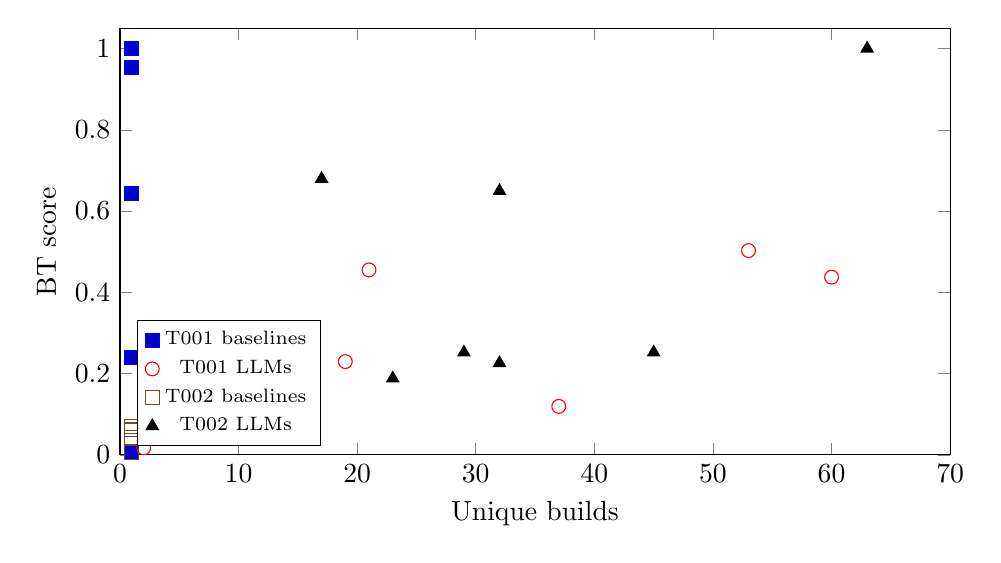
\begin{tikzpicture}
\begin{axis}[
width=\columnwidth, height=7cm,
xlabel={Unique builds},
ylabel={BT score},
xmin=0, xmax=70, ymin=0, ymax=1.05,
legend style={at={(0.02,0.02)},anchor=south west,font=\scriptsize},
]
\addplot+[only marks, mark=square*, mark size=2.5pt] coordinates {
(1,1.0000) (1,0.9541) (1,0.6426) (1,0.2388) (1,0.0054)
};
\addlegendentry{\tOne{} baselines}
\addplot+[only marks, mark=o, mark size=2.5pt] coordinates {
(53,0.5028) (21,0.4553) (60,0.4373) (19,0.2296) (37,0.1193) (3,0.0656) (9,0.0564) (2,0.0173)
};
\addlegendentry{\tOne{} LLMs}
\addplot+[only marks, mark=square, mark size=2.5pt] coordinates {
(5,0.0926) (1,0.0698) (1,0.0614) (1,0.0426) (1,0.0066)
};
\addlegendentry{\tTwo{} baselines}
\addplot+[only marks, mark=triangle*, mark size=2.5pt] coordinates {
(63,1.0000) (17,0.6793) (32,0.6496) (6,0.2520) (29,0.2520) (45,0.2520) (32,0.2258) (23,0.1882)
};
\addlegendentry{\tTwo{} LLMs}
\end{axis}
\end{tikzpicture}
\caption{Build diversity vs.\ BT score across both tournaments.}
\label{fig:diversity_scatter}
\end{figure}

\section{Discussion}

\paragraph{Comprehension vs.\ reasoning.}
The flip from \tOne to \tTwo implicates \emph{comprehension and representation} more than an absence of strategic capability.
In \tOne, LLMs must translate qualitative descriptions into an implicit quantitative model; baselines that encode numeric heuristics dominate.
In \tTwo, providing formulas and examples makes the same optimization problem tractable, and LLMs surpass baselines decisively.
The bottleneck in \tOne is not that LLMs ``cannot reason'' but that they cannot reliably extract quantitative structure from vague natural-language descriptions.

\paragraph{Feedback and adaptation.}
Within-series feedback is useful (Table~\ref{tab:t2_adapt}), but it is not the only path to success.
Codex adapts in 91\% of losses and wins with the highest build diversity.
Flash adapts in only 38\% of losses but achieves the highest per-adaptation win rate (76\%).
Adaptation rate and build diversity are not sufficient statistics for final rank; what matters is whether the agent converges to strong builds, by whatever path.

\paragraph{Meta knowledge.}
The meta block in \tTwo provides a strong initialization that \tOne lacks.
Notably, the injected meta context was itself imperfect: it was computed on a filtered subset of \tOne data, and all five builds showed 100\% win rate on small samples (4--22 games), somewhat overstating their true strength.
Despite this noise, the meta block was sufficient to shift the regime: LLM-vs-baseline series win rate increased from 37.50\% to 89.75\%.
Since \tTwo changes multiple variables simultaneously, we cannot attribute this reversal to meta context alone (see Limitations).

\paragraph{Price--performance paradox.}
Across both tournaments, Claude Opus---the most expensive Claude tier at the time of evaluation---is consistently the weakest Claude by Elo.
Opus loses 0--10 to Sonnet in both \tOne and \tTwo.
In \tOne, Sonnet is the strongest Claude by BT (0.066 vs.\ Opus's 0.017).
In \tTwo, Opus and Sonnet share BT=0.252 but Opus has the lowest Elo among Claude models (1526 vs.\ Sonnet's 1709 and Haiku's 1553).
This suggests that model cost and general helpfulness tuning do not imply strategic robustness under this benchmark.

\paragraph{Non-transitivity as a meta-complexity indicator.}
The appearance of 12 strict 3-cycles in \tTwo (vs.\ 0 in \tOne) suggests that adaptation creates a richer strategic landscape.
Under one-shot play, the meta collapses to ``stack ATK''; under adaptation, counter-picking introduces genuine rock--paper--scissors dynamics where no single build dominates all others.

\section{Limitations}
\label{sec:limits}

\begin{enumerate}[leftmargin=*]
\item \textbf{Multiple simultaneous interventions in \tTwo.}
\tTwo introduces four major changes at once (exact formulas, meta context, per-game adaptation with winner lock, structured output schema), so we cannot attribute the performance reversal to any single factor.
Future ablations (Section~\ref{sec:future}) will isolate each intervention.

\item \textbf{Prompt dependence is part of the construct.}
The large \tOne$\to$\tTwo swing highlights that ``strategy'' and ``prompt engineering'' interact tightly.
This is a feature, not a bug: Moreau Arena intentionally stresses rule comprehension, and the prompt sensitivity itself is a measurable result.
However, we have not yet run a prompt sensitivity suite to quantify how much wording variation within each protocol affects rankings.

\item \textbf{Statistical resolution.}
Each pair plays 10 series.
Confidence intervals overlap for several adjacent LLM ranks (Tables~\ref{tab:t1_rank}--\ref{tab:t2_rank}); finer-grained ordering would benefit from more series.
Three agents share BT=0.252 in \tTwo, and their relative ordering is not statistically resolved.

\item \textbf{Decoding settings.}
Temperature and sampling differ across provider defaults and were not swept.
A controlled decoding ablation may change relative performance among closely ranked LLMs.

\item \textbf{No human baseline.}
We do not yet include human players, which would provide a useful anchor for interpreting LLM performance.

\item \textbf{Meta context fidelity.}
The \tTwo meta block was extracted from a filtered subset of \tOne data (excluding floor baselines), yielding uniformly 100\% win rates on small samples.
The injected builds are strong but their stated win rates overestimate true population rates.
We document the exact injected text in Appendix~\ref{app:t2_prompt}.
\end{enumerate}

\section{Future Work}
\label{sec:future}

The most important next step is a series of ablations to isolate each \tTwo intervention:
(a) exact formulas only (no meta, no adaptation);
(b) meta context only (no adaptation);
(c) adaptation only (vague prompt).
These ablations will support causal rather than correlational claims about which scaffolding component drives the performance reversal.

We plan to formalize Moreau Arena as a \emph{tiered measurement battery} with four standardized tracks:
Track~A (one-shot, as in \tOne),
Track~B (feedback adaptation, as in \tTwo),
Track~C (meta-conditioned without adaptation),
and Track~D (tool-augmented, where agents may use a calculator or limited simulator).
Each track measures a distinct axis of strategic competence; results should not be compared across tracks.

Additional planned extensions include:
enabling the auto-balancer between tournaments to study non-stationary metas;
adding human baselines (competitive gamers given the same prompt and time budget);
analyzing reasoning traces to understand \emph{why} some models explore more broadly;
running a prompt sensitivity suite (3--5 semantically equivalent prompts) and reporting rank stability (Kendall $\tau$) across prompt variants;
and computing formal non-transitivity statistics (3-cycle mass, Condorcet winner existence) as the agent pool grows.

\section{Ethics and Responsible Benchmarking}

Moreau Arena is designed to support responsible benchmarking:
(i) a newly authored ruleset to reduce contamination risk,
(ii) deterministic execution under hashed seeds (the simulator is deterministic given the recorded actions and the seed; LLM sampling may be stochastic, so reproducibility is achieved by recording actions, decoding settings, and seeds),
(iii) a frozen configuration snapshot for reproducibility,
and (iv) a planned auto-balancing mechanism to mitigate overfitting to a static meta in long-running leaderboards.
We present results as descriptive measurements of capability and failure mode, avoiding normative claims about intent or deception.
Strong performance under heavy scaffolding (\tTwo) does not imply robust decision-making in safety-critical domains; we recommend reporting results under multiple prompt regimes.

\section{Conclusion}

Two tournaments over the same 13 agents and frozen game configuration reveal a sharp boundary condition for LLM strategic reasoning.
Under a vague, one-shot prompt with no feedback (\tOne, 779 series), handcrafted baselines dominate and LLMs exhibit qualitative traps---most notably the WIL trap, where compositional failure (large-looking percentages modulating rare events) leads to systematically dominated builds.
When mechanics are explicit, examples are provided, and feedback is allowed (\tTwo, 780 series), the leaderboard reverses completely: every LLM outranks every baseline.

The most important result is the gap itself.
It suggests that for strategic tasks, the limiting factor is often not the existence of reasoning machinery but whether the task representation and feedback channel allow that machinery to operate.
GPT-5.2-Codex's leap from rank~9 to rank~1 illustrates this vividly: the same model, under different scaffolding, goes from near-worst to overall winner.

We release the complete prompts, configuration hash, match records, and analysis code to support reproducibility and follow-up studies.

\section*{Use of Generative AI Tools (Disclosure)}
Generative AI language tools were used (i) as \emph{subjects} in the tournament experiments analyzed; and (ii) as writing aids for drafting and editing.
No AI system is listed as an author.
All claims, data verification, interpretations, and final wording were selected and reviewed by the human author, who takes responsibility for the content and any remaining errors.

\section*{Acknowledgements}
I thank the Round Table collaborative research group for methodological discussions that shaped this work, and the model providers whose APIs made the experiments possible.
Any errors or misinterpretations are my own.

\begin{thebibliography}{99}

\bibitem{bradley_terry}
R.~A.~Bradley and M.~E.~Terry.
\newblock Rank analysis of incomplete block designs: {I}. {T}he method of paired comparisons.
\newblock \emph{Biometrika}, 39(3/4):324--345, 1952.

\bibitem{pluribus}
N.~Brown and T.~Sandholm.
\newblock Superhuman {AI} for multiplayer poker.
\newblock \emph{Science}, 365(6456):885--890, 2019.

\bibitem{cicero}
A.~Bakhtin et~al.
\newblock Human-level play in the game of {D}iplomacy by combining language models with strategic reasoning.
\newblock \emph{Science}, 378(6624):1067--1074, 2022.

\bibitem{nle}
H.~K{\"u}ttler et~al.
\newblock The {N}et{H}ack {L}earning {E}nvironment.
\newblock In \emph{NeurIPS}, 2020.

\bibitem{procgen}
K.~Cobbe et~al.
\newblock Leveraging procedural generation to benchmark reinforcement learning.
\newblock In \emph{ICML}, 2020.

\bibitem{helm}
P.~Liang et~al.
\newblock Holistic evaluation of language models.
\newblock \emph{arXiv preprint arXiv:2211.09110}, 2022.

\bibitem{chatbot_arena}
L.~Zheng et~al.
\newblock Judging {LLM}-as-a-judge with {MT}-{B}ench and {C}hatbot {A}rena.
\newblock \emph{arXiv preprint arXiv:2306.05685}, 2023.

\bibitem{mmlu}
D.~Hendrycks et~al.
\newblock Measuring massive multitask language understanding.
\newblock In \emph{ICLR}, 2021.

\bibitem{gsm8k}
K.~Cobbe et~al.
\newblock Training verifiers to solve math word problems.
\newblock \emph{arXiv preprint arXiv:2110.14168}, 2021.

\bibitem{arc}
F.~Chollet.
\newblock On the measure of intelligence.
\newblock \emph{arXiv preprint arXiv:1911.01547}, 2019.

\bibitem{bigbench}
A.~Srivastava et~al.
\newblock Beyond the imitation game: Quantifying and extrapolating the capabilities of language models.
\newblock \emph{arXiv preprint arXiv:2206.04615}, 2022.

\end{thebibliography}

\appendix

\section{Tournament~001 prompt}\label{app:t1_prompt}

The following reproduces the prompt shown to every LLM in Tournament~001 (from \texttt{build\_prompt(opponent\_animal=None, banned=[])} in \texttt{src/moreau/llm\_agent.py}; line breaks adjusted for page width, no characters altered).

\begingroup
\small
\begin{verbatim}
You are designing a creature for Moreau Arena,
a 1v1 combat game on an 8x8 grid.

RULES:
- Allocate exactly 20 stat points across 4 stats:
  HP, ATK, SPD, WIL (each minimum 1)
- Stat formulas:
    max_hp = 50 + 10 * HP
    base_dmg = floor(2 + 0.85 * ATK)
    dodge = SPD * 2.5%  (capped 30%)
    resist = min(60%, WIL * 3.3%)
- Closing Ring starts at tick 30, dealing increasing
  damage to creatures on outer tiles
- Abilities proc randomly each tick based on
  proc chance

AVAILABLE ANIMALS:
  BEAR - Passive: Fury Protocol - gains +ATK
    when damaged
    Abilities: Berserker Rage: +ATK buff for
    3 ticks (3.5% proc); Last Stand: 2x damage
    when below 15% HP (single charge, 3.5% proc)
  BUFFALO - Passive: Thick Hide - takes reduced
    damage
    Abilities: Thick Hide: Reduces incoming damage
    for 1 tick (4.5% proc); Iron Will: Survives
    a killing blow at 1 HP (single charge, 3.5%
    proc)
  BOAR - Passive: Charge - bonus damage on
    first hit
    Abilities: Stampede: AoE damage + knockback
    (4.5% proc); Gore: 0.6x damage but ignores
    dodge (3.5% proc)
  TIGER - Passive: Ambush Wiring - high dodge,
    first-strike advantage
    Abilities: Pounce: +70% damage + stun (4.5%
    proc); Hamstring: -55% SPD, -10% dodge for
    4 ticks (4.5% proc)
  WOLF - Passive: Pack Sense - bonus to ability
    proc chance
    Abilities: Pack Howl: +ATK buff for 4 ticks
    (4.5% proc); Rend: DoT bleed for 3 ticks
    (4.5% proc)
  MONKEY - Passive: Primate Cortex - adaptive,
    copies opponent abilities
    Abilities: Chaos Strike: Random damage
    multiplier 0.5x-2.0x (4.5% proc); Mimic:
    Copies opponent's last ability (3.5% proc)

Choose an animal and allocate 20 stat points.
Respond ONLY in this exact format:
ANIMAL HP ATK SPD WIL
Example: BOAR 8 8 3 1
\end{verbatim}
\endgroup

\noindent All LLM calls used \texttt{max\_tokens=64} with a 120-second hard timeout.
Invalid outputs triggered one retry; persistent failures fell back to GreedyAgent (\texttt{boar 8/8/3/1}).

\section{Tournament~002 prompt additions}\label{app:t2_prompt}

\tTwo augments the \tOne prompt with three blocks: (1) explicit numerical formulas for all passives and abilities, (2) metagame context automatically extracted from \tOne match records, and (3) a JSON output schema enforced via provider-specific structured output APIs.

\paragraph{Exact numerical formulas (excerpt).}
\begingroup
\small
\begin{verbatim}
STAT FORMULAS:
  max_hp = 50 + 10 * HP
  base_dmg = floor(2 + 0.85 * ATK)
  dodge_chance = min(30%, SPD * 2.5%)
  ability_resist = min(60%, WIL * 3.3%)
  ability_proc_bonus = WIL * 0.08% (additive)

PASSIVE DETAILS:
  BEAR - Fury Protocol: +1 ATK per hit taken
    (permanent, stacks)
  BUFFALO - Thick Hide: incoming damage
    reduced by 15%
  BOAR - Charge: first attack deals 1.5x damage
  TIGER - Ambush Wiring: +10% base dodge,
    attacks first on tick 1
  WOLF - Pack Sense: +1.5% additive to all
    ability proc rates
  MONKEY - Primate Cortex: 20% chance to copy
    opponent's last proc
\end{verbatim}
\endgroup

\paragraph{Meta context (exact text injected into every \tTwo prompt).}
The following was generated automatically by \texttt{meta\_extractor.py}, which filters out floor baselines (RandomAgent, HighVarianceAgent) and ranks remaining builds by win rate on the filtered subset.
All five builds show 100\% win rate on their respective subsamples; game-level win rates across all agents are lower (80--100\%).

\begingroup
\small
\begin{verbatim}
META CONTEXT (top builds from previous tournament,
ranked by win rate):
  1. BEAR 8/8/3/1  - 100% win rate (22 games)
  2. BEAR 8/10/1/1 - 100% win rate (19 games)
  3. BEAR 10/8/1/1 - 100% win rate (11 games)
  4. WOLF 7/10/2/1 - 100% win rate (4 games)
  5. BEAR 9/9/1/1  - 100% win rate (4 games)
\end{verbatim}
\endgroup

\paragraph{JSON output schema.}
\begingroup
\small
\begin{verbatim}
Respond ONLY with valid JSON:
{"animal":"BEAR","hp":3,"atk":14,"spd":2,"wil":1}

Rules: animal in {BEAR,BUFFALO,BOAR,TIGER,WOLF,
MONKEY}, hp+atk+spd+wil=20, each stat >= 1.
\end{verbatim}
\endgroup

\noindent Structured output was enforced via provider-specific APIs (Anthropic \texttt{tool\_use}, OpenAI \texttt{json\_schema}, Google \texttt{response\_schema}, xAI JSON mode).
Regex fallback was available but triggered zero times across all 780 \tTwo series.

\end{document}
